%%% THIS IS A WORK IN PROGRESS! %%%

\documentclass{article}
\usepackage[utf8]{inputenc}
\usepackage[german]{babel} % Silbentrennung, Anführungszeichen usw.
%\usepackage[babel,german=quotes]{csquotes}

\usepackage{url}
\usepackage{listings}
\usepackage{color}
\usepackage{graphicx}
\usepackage[a4paper,margin=1in]{geometry}

\usepackage{mathptmx}% http://ctan.org/pkg/mathptmx

\usepackage{array}
\usepackage{multirow}


\definecolor{mygreen}{rgb}{0,0.2,0}
\definecolor{mygray}{rgb}{0.95,0.95,0.95}
\definecolor{mymauve}{rgb}{0.58,0,0.82}

\lstdefinelanguage{mylog}{
  comment=[l]{//},
  morecomment=[s]{/*}{*/}
}

\title{GeoGebra Automatisierte Begründungwerkzeuge\\ \large Ein Tutorial}
\author{Zolt\'an Kov\'acs, Tom\'as Recio und M. Pilar V\'elez\\
Übersetzt von Katharina Schiffler\\
\textbf{work in progress}
}
%\date{January 2017}

\begin{document}
\lstset{
  basicstyle=\ttfamily,
  columns=fullflexible,
  keepspaces=true,
  breaklines=true,
  backgroundcolor=\color{mygray},
  keywordstyle=\color{blue},
  stringstyle=\color{mymauve},
  ndkeywordstyle=\color{red},
  commentstyle=\color{mymauve},
  identifierstyle=\color{mygreen}
}
%\tolerance10000

\maketitle

\section{Einführung}

Das Softwaretool GeoGebra (\url{http://www.geogebra.org}) ist geeignet zur Unterstützung des Unterrichts der zweidimensionalen euklidischen Geometrie Theorien mit symbolischen Berechnungen. Zu diesem Zweck wurden einige Werkzeuge für den automatischen Beweis und zur Entdeckung von geometrischen Lehrsätzen entwickelt.

Die neuen Technologien im Klassenzimmer befinden sich noch in einer experimentellen Phase. Dieses Dokument fasst die technischen Möglichkeiten zusammen und zeigt auch einige Beispiele.

\section{Starting GeoGebra}

GeoGebra ist auf vielen Plattformen verfügbar, wie zum Beispiel
\begin{itemize}
    \item Computer mit verschiedenen Betriebssystemen
    \item Tablets, und
    \item Smartphones.
\end{itemize}
Darüber hinaus sind eingebettete GeoGebra Applets auf Websites verfügbar, speziell auf GeoGebra Materials (\url{https://www.geogebra.org/materials/}) mit Millionen kostenlos verfügbarer Unterrichtsmaterialien.

Die verfügbaren Werkzeuge können unter Umständen variieren. Auch die Benutzererfahrung kann auf den verschiedenen Plattformen unterschiedlich sein: Die symbolischen Berechnungen können ein hohes Ausmaß an Kalkualtionen benötigen und die unterliegenden Hardware- und Softwarekomponenten unterstützen möglicherweise nicht alle Schritte vollständig.

Die vorgeschlagene Plattform für Klassen kann variieren. Die schnellsten Resultate können mit schnellen Computern erzielt werden, aber in diesem Fall muss die Software vom Benutzer heruntergeladen und installiert werden. Manche Beispiele in diesem Tutorial funktionieren unter Umständen nur in der \glqq{}Desktop\grqq{} Version (welche für Microsoft Windows, Apple Macintosh und Linux Computer verfügbar ist). Auf der anderen Seite benötigt die ``Web'' Version keine Installation durch den Benutzer: Diese funktioniert mit einem aktuellen Web Browser und die Lehrerin/der Lehrer kann zum Beispiel eine Liste von Beispielen als GeoGebra Applets für die Klasse unter Verwendung von GeoGebra Materials vorbereiten. Die ``Web'' Version ist allerdings langsamer: Die symbolische Berechnung kann etwas langsamer sein.

GeoGebra funktioniert mittlerweile auch auf Tablets und Smartphones. In manchen Fällen können diese Plattformen schnellere Ergebnisse liefern als die Web Version, aber der kleinere Bildschirm könnte die Benutzer davon abhalten, geometrische Lehrsätze im Detail zu untersuchen. Lehrerinnen und Lehrer sollen bestärkt werden, mit dem Umgang dieser modernen Hilfsmittel zu experimentieren, aber der Einsatz für automatische Beweisführung ist noch nicht erforscht.

An den Werkzeugen zur automatischen Beweisführung wird kontinuierlich gearbeitet. Es ist zu bevorzugen, immer die aktuellste Version zu verwenden. Ein wöchentliches Update kann generell für alle Versionen empfohlen werden, abgesehen vom Mac App Store, welcher ungefähr monatlich aktualisiert wird. Die Liste der neuesten Änderungen kann auf \url{http://dev.geogebra.org/trac/timeline}---eingesehen werden -das ist nur für fortgeschrittene Benutzer und Entwickler. 

\section{Automatische Beweisführung Werkzeuge}

Automatische Beweisführung Werkzeuge sind eine Sammlung von GeoGebra Werkzeugen und Befehlen zur Mutmaßung, Entdeckung, Abstimmung und Beweis geometrischer Axiome in einer dynamischen geometrischen Konstruktion.

Am Anfang muss der Benutzer eine geometrische Figur mit bestimmten Werkzeugen auf dem Hauptfenster in GeoGebra zeichnen. Nach der Konstruktion der Figur kann GeoGebra auf verschiedene Arten die geometrischen Eigenschaften mit verschiedenen Werkzeugen und Einstellungen prüfen:
\begin{enumerate}
    \item Mit \textit{freie Objekte ziehen} ihre abhängigen Objekte können sichtbar erforscht werden.
    \item Das \textit{Beziehung} Werkzeug hilft beim Vergleichen von Objekten und erkennen von Beziehungen.
    \item Mit dem Setzen der  \textit{Spur} eines konstruierten Objektes mit/ohne Bewegung eines Objektes wird sichtbar wenn seine vorhergehenden Objekte geändert werden.
    \item Das \textit{Ortslinie} Werkzeug zeigt die Spur eines Objektes für alle möglichen Posititonen eines vorhergehenden Objektes (wenn es sich auf einem Pfad bewegt).
    \item Mit dem Eintippen von \texttt{Beziehung} oder \texttt{Ortslinie} Befehl in der GeoGebra Befehlszeile können genauere Informationen ausgewählt werden. 
\end{enumerate}
Diese Methoden sind normalerweise bekannt in der GeoGebra community, deshalb sind sie gut dokumentiert und es können einige Beispiele auf GeoGebra Materials (\url{https://www.geogebra.org/materials/}) gefunden werden. Auf der anderen Seite bietet GeoGebra zurzeit auch symbolische automatische Beweisführung Werkzeuge für vermutete geometrische Eigenschaften:
\begin{enumerate}
\setcounter{enumi}{5}
    \item Beziehung Werkzeug und Befehl können zum symbolischen Nachrechnen verwendet werden,
    \item Der \texttt{Ortsliniengleichung} Befehl berechnet das Ergebnis der Ortsliniengleichung mit dem Zeigen der algebraischen Gleichung der graphischen Darstellung genauer.
    \item Der \texttt{Ortsliniengleichung} Befehl kann implicit loci prüfen.
    \item Der \texttt{Einhüllende} Befehl berechnet die Gleichung der Tangente mehrerer Objekte während ein bestimmter Vorgänger sich auf einer Bahn bewegt.
\end{enumerate}

\subsection{Einfache und schwierige Werkzeuge}

GeoGebra liefert die obenstehenden schwierigen Methoden um geometrische Theorien zu unterstützen. Diese Icons sind als schwierige Werkzeuge gedacht, weil sie aufgrund ihrer einfachen Benutzung direkt in der Klasse gezeigt werden können. Es gibt auch andere Wege, um mehr über den mathematischen Hintergrund zu lernen oder einfach zur Fehleranalyse. Diese einfachen Methoden sind im Zusatz aufgelistet und daher nicht empfohlen für den direkten Einsatz mit Schülerinnen und Schülern.

Offensichtlich sind einige der aufgelisteten Methoden einfach und andere schwierige. Bei der Befehlszeile in GeoGebra kann überlegt werden als ein schwierigerer Weg für die meisten Benutzer. Daher kann eine Lehrerin/ein Lehrer zuerst die einfacheren Methoden zeigen und nach einiger Erfahrung der Schülerinnen und Schüler die schwierigeren. 

\subsection{Werkzeuge mit symbolischer Unterstützung}

Wie oben erwähnt liefern einige automatische Beweisführung Werkzeuge symbolische Unterstützung. Dieses Feature erlaubt die Verifizierung einem mathematisch rigorosem Weg allgemeine Aussagen der Elementargeometrie, die vom Benutzer vermutet werden.

Ein allgemeiner Hinweis, dass der Benutzer sollte GeoGebra zur Inbetriebnahme mit``Grafikrechner'' Modus starten. Diese Einstellung zeigt die Bezeichnung auf jedem neu hinzugefügten Objekt. Das kann für Beziehungswerkzeug und -befehl entscheidend sein, wenn die verschiedenen Beziehungen ausgewertet werden. 

In den meisten Fällen sind die Achsen nicht wirklich notwendig: Diese können ausgeschaltet werden, wenn das \textit{Bewegen} Werkzeug aktiv ist. (das ist das linke Icon, das einen Cursor zeigt) mit rechtsklickc in der \textit{Grafik Ansicht} und Auswahl der \textit{Achsen} Einstellung.

In einigen Fälle ist es nicht notwendig, die \textit{Algebra Ansicht} anzuzeigen. Wenn die Gleichungen der impliziten Kurven nicht im Detail betrachtet werden,  kann dies auch durch die Änderung der Bezeichnung erreicht werden, sodass auch der Wert angezeigt wird. (Um das durchzuführen, muss ein Rechtsklick und die Auswahl \textit{Objekt Eigenschaften} durchgeführt werden, der Benutzer muss  \textit{Beschriftung anzeigen} zu \textit{Wert} an dem  \textit{Basis} auswählen.)

GeoGebra Applets können komfortabel genutzt werden, wenn sie auf GeoGebra Materials hochgeladen  sind.
Wenn die Algebra Ansicht verwendet wird, kann es hilfreich sein, die Weite zu vergrößern, bevor das Applet auf GeoGebra Materials hochgeladen wird. Sonst könnte es schwierig für den Benutzer sein, die Befehle einzugeben. Nach dem hochladen in GeoGebra Materials ist es wichtig, die Funktionen des Applets  \textit{Erweiterte Einstellungen},  \textit{Zeige Werkzeugleiste} und \textit{Zeige Befehlszeile} zu überprüfen. Danach sollte eine adäquate Größe für das Applet gewählt werden.


\subsubsection{Das Beziehungswerkzeug und Befehle}

GeoGebra's Beziehungswerkzeug und Befehle zeigt ein Fenster, das dem Benutzer Informationen über die Beziehung zwischen zwei oder mehr Objekten gibt.
Dieser Befehl erlaubt dem Benutzer, numerisch herauszufinden, ob (für die gezeichnete Konstruktion mit zugehörigen Koordinaten)
\begin{itemize}
    \item zwei Geraden normal aufeinander stehen,
    \item zwei Geraden parallel sind,
    \item zwei (oder mehr) Objekte (Punkte, Streckenlängen, Polygonflächen) gleich sind,
    \item ein Punkt auf einer Linie oder Kurve liegt,
    \item eine Gerade eine Tangent oder eine Passante einer Kurve ist,
    \item drei Punkte kollinear sind,
    \item drei Geraden übereinstimmend sind (oder parallel),
    \item vier Punkte auf einer Kreisbahn liegen (oder kollinear sind).
\end{itemize}
Manche dieser Überprüfungen können auch symbolisch ausgeführt werden, also der Satz kann generell verifiziert werden (mit beliebigen Koordinaten) und nicht nur für die gezeichnete konkrete Konstruktion.

Mit der Verwendung des Beziehungs \textit{werkzeug} muss der Benutzer auf zwei Objekte klicken um die Mitteilungsbox zu sehen. Alternativ können zwei, drei oder vier Objekte mit dem Auswahlrechteck ausgewählt werden, um die Mitteilungsbox zu erhalten. Um nicht ungewollte Objekte im Applet auszuwählen ist es möglich, diese von der Auswahl auszunehmen, indem man mit einem Rechtsklick und der Auswahl \textit{Objekt Eigenschaften} \textit{Erweitert} auswählt und das Häkchen bei \textit{Auswahl erlaubt}entfernt.

Bei der Verwendung des Beziehungs \textit{befehls} gibt der Benutzer eine der folgenden Formlen in die Befehlszeile ein:
\begin{itemize}
    \item \texttt{Beziehung[ <Objekt>, <Objekt> ]}
    \item \texttt{Beziehung[ \{ <Objekt>, <Objekt> \} ]}
    \item \texttt{Beziehung[ \{ <Objekt>, <Objekt>, <Objekt> \} ]}
    \item \texttt{Beziehung[ \{ <Objekt>, <Objekt>, <Objekt>, <Objekt> \} ]}
\end{itemize}

Wenn die Mitteilungsbox eines oder mehrere zutreffende numerische Aussagen zu dem Objekt zeigt, gibt es unter Umständen eine Schaltfläche  ``Mehr$\ldots$'' , welche die symbolische Unterstützung für die gegebene Aussage zeigt. Bei Klick auf ``Mehr $\ldots$'', wird in Kürze die numerische Aussage zu einer allgemeinen Aussage aktualisiert.

\paragraph{Beispiel (Thaleskreis)}
\begin{center}
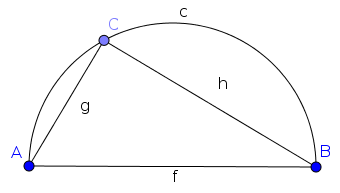
\includegraphics[scale=0.5]{Relation-example}
\end{center}
\begin{enumerate}
    \item Mit dem \textit{Strecke} Werkzeug wird $AB$ konstruiert.
    \item Mit der Auswahl \textit{Halbkreis durch zwei Punkte} Werkzeug wird $c$ erstellt.
    \item Der Punkt $C$ wird auf $c$ erstellt.
    \item Konstruieren Sie die Strecken $AC$ und $BC$ und benennen Sie diese $g$ und $h$.
    \item Vergleichen Sie $g$ und $h$ unter Verwendung des Beziehungswerkzeugs durch Anklicken von $g$ und $h$, oder durch Eintippen von \texttt{Beziehung[g,h]} in der Befehlszeile. Die folgende Mitteilung wird angezeigt:
    \begin{center}
    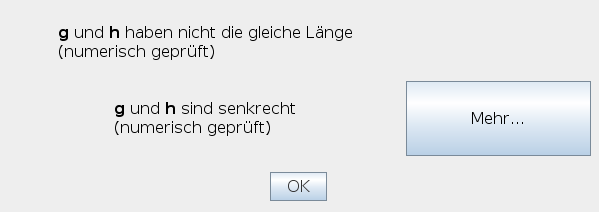
\includegraphics[scale=0.5]{Relation-example-Relation1-de}
    \end{center}
    \item Klicken Sie auf ``Mehr$\ldots$''--- die Mitteilung wird sich wie folgt ändern:
    \begin{center}
    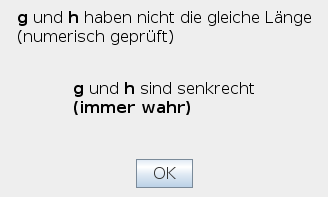
\includegraphics[scale=0.5]{Relation-example-Relation2-de}
    \end{center}
    
\end{enumerate}

Beachten Sie, dass Beziehung (Schritt 5) sucht nach Beziehungen zwischen $g$ und $h$ von den Koordinaten und Gleichungen abhängig von der gezeichneten Konstruktion. Durch Klicken auf ``Mehr$\ldots$'' (Schritt 6) kann verifiziert werden, dass $g$ und $h$ normal aufeinander stehen und für alle Punkte kann $A$ und $B$ kann man Schritt 1 auswählen.

Beziehung zwischen bestimmten Objekten kann unter bestimmten Bedingungen wahr sein, aber nicht zwingend  ``immer''. In diesen Fällen werden genug Voraussetzungen angezeigt. Sonst zeigt GeoGebra nur die Aussage  ``unter bestimmten Voraussetzungen''. Das muss als ``allgemein wahr'' verstanden werden, aber in manchen Einzelfällen (welche eine`minimale Anzahl von Fällen' ist, verglichen mit den allgemeinen Fällen) kann die Aussage falsch sein.

Das symbolische Ergebnis der Beziehung kann auch negativ sein, auch wenn die numerische Überprüfung positiv ist. Zum Beispiel, wenn man zwei Punkte $P=(0,0)$und $Q=(0,0)$ definiert, kann die Beziehung diese numerisch vergleichen, aber das symbolische Ergebnis kann ergeben, dass``$P$ und $Q$ gleich sind (aber nicht allgemein wahr)''.

Eine komplette Übersicht der verschiedenen Ergebnisse der Beziehung könnene im Anhang gefunden werden. \ref{Erklaerungstabelle} auf der Seite \pageref{Erklaerungstabelle}.

\subsubsection{Die Ortsliniengleichung \texttt{Ortsliniengleichung} Befehl}

Dieser Befehl berechnet die Gleichung einer Ortslinie und zeichnet diese als implizite Kurve. Es gibt zwei Möglichkeiten der Nutzung:

\begin{itemize}
\item\textbf{Explizite Ortslinie.}
Gegeben ist ein Anfangspunkt $\cal{I}$ auf einer Strecke $\cal{P}$, einige Konstruktionsschritte und ein Endpunkt $\cal O$. Die Aufgabe ist, die Gleichung von $\cal E$ of $\cal O$ zu bestimmen, wenn sich  $\cal I$ auf $\cal P$ bewegt, und dann  $\cal E$ zu bestimmen. $\cal I$ ist für gewöhnlich \textit{beweger} genannt, $\cal O$ ist die \textit{Spur}. $\cal E$ heißt \textit{Ortsliniengleichung} und ihre grafische Visualisierung ist die \textit{Ortslinie}.

Die Schreibweise des Befehls ist:
\begin{center}
    \texttt{Ortsliniengleichung[ <Punkt Spur>, <Punkt Beweger> ]}.
\end{center}

\paragraph{Beispiel}
\begin{center}
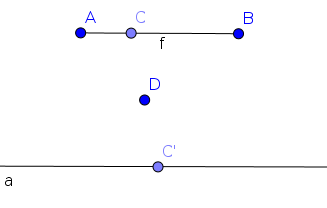
\includegraphics[scale=0.5]{LocusEquation-example-explicit}
\end{center}
\begin{enumerate}
    \item Unter Verwendung des \textit{Strecke} Werkzeug wird $AB$ konstruiert. Es wird eine automatische Strecke $f$ konstruiert.
    \item Setzen Sie Punkt $C$ auf $f$.
    \item Erstellen Sie Punkt $D$ mit dem \textit{Punkt} Werkzeug.
    \item Mit dem \textit{über Punkt spiegeln} Werkzeug spiegeln Sie $C$ über $D$. Damit erstellen Sie Punkt $C'$.
    \item Geben Sie \texttt{Ortsliniengleichung[C',C]} in die Befehlszeile ein. Nun wird die implizite Kurve $a$ berechnet und gezeichnet. Das sollte eine Strecke (das Spiegelbild von $f$ über $D$ sein), aber GeoGebra zeichnete $f$ als Gerade statt einer Strecke (aus algebraischen geometrischen Gründen), da das Spiegelbild ebenfalls eine Gerade ist.
    \item Versuchen Sie, die verschiebbaren Objekte zu ziehen. Es kann gezeigt werden, dass das Spiegelbild einer Strecke über einen Punkt immer parallel zum Urbild ist.
\end{enumerate}

\item \textbf{Implizite Ortslinie.}
Gegeben ist ein Anfangspunkt $\cal I$, entweder als beliebiger Punkt oder auf einer Strecke $\cal P$. Es sind auch einige Konstruktionsschritte gegeben. Der Benutzer behauptet eine Boolsche Bedingung $\cal C$ auf einige Objekte der Konstruktion. Die Aufgabe ist, eine Gleichung $\cal E$ für alle Punkte $\cal{I}'$ aufzustellen, sodass $\cal{I}=\cal{I}'$,  $\cal{C}$ erfüllt. Wieder heißt  $\cal{E}$ Ortsliniengleichung und ihre grafische Interpretation ist die Ortslinie.

Die Schreibweise des Befehls ist:
\begin{center}
    \texttt{Ortsliniengleichung[ <Boolscher Ausdruck>, <Punkt> ]}.
\end{center}

%\vfill\eject %% no idea how to do it elegantly

\paragraph{Beispiel}
\begin{center}
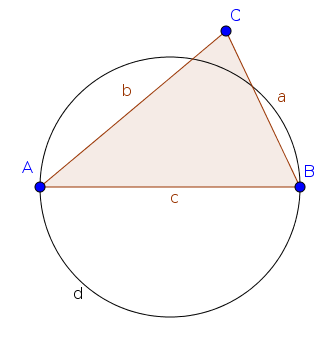
\includegraphics[scale=0.5]{LocusEquation-example-implicit}
\end{center}
\begin{enumerate}
    \item Mit dem \textit{Polygon} Werkzeug wird ein Dreieck $ABC$ konstruiert.Die Strecken $a$, $b$ und $c$ werden automatisch von GeoGebra erstellt.
    \item Es wird \texttt{Ortsliniengleichung a\^{}2+b\^{}2==c\^{}2,C]} in der Werkzeugleiste eingegeben. Jetzt wird die implizite Kurve $d$ berechnet und gezeichnet, welche wie ein Kreis aussieht.
    Bedenken Sie, dass \textit{zwei} gleiche Zeichen eingegeben werden müssen; eine andere Möglichkeit ist, $\stackrel{?}{=}$ zu verwenden. (durch anklicken von \framebox{$\alpha$} Icon, oder durch Einfügen des Symbols von einer externen Applikation mit Copy and Paste).
    \item Versuchen Sie nun, die beweglichen Objekte zu ziehen. Es kann gezeigt werden, dass wenn $C$ auf einem Kreis liegt, dessen Durchmesser auf $AB$ liegt, wegen der rechtwinkeligen Eigenschaft des Dreiecks---$a^2+b^2=c^2$ gilt.
\end{enumerate}

\end{itemize}

Eine Boolsche Bedingung kann sein:
\begin{itemize}
\item Eine Gleichung mit der Bezeichnung der Strecken, e.g.~\texttt{a\^{}2+b\^{}2==c\^{}2}.
\item Eine Gleichheit von zwei Geometrischen Objekten, e.g.~\texttt{A==B}. Beachten Sie, dass \textit{zwei} gleiche Zeicehn eingegeben werden müssen; es gibt auch andere Möglichkeiten
\begin{itemize}
    \item $\stackrel{?}{=}$ (durch Anklicken des \framebox{$\alpha$} Icon, oder durch Einfügen des Symbols von einer externen Applikation mit Copy and Paste.
    \item Alternativ, \texttt{SindGleichl[A,B]} für die gesamte Boolsche Bedingung.
\end{itemize}
\item Eine Überprüfung, ob zwei geometrische Objekte kongruent sind, e.g.~\texttt{SindKongruent[c,d]}.
\item Eine Überpüfung, ob ein Punkt auf einer Strecke, einer Gerade oder einem Kreis liegt, e.g.~\texttt{A$\in$c}.
\item Eine Überprüfung, ob zwei Geraden oder Strecken parallel sind, e.g.~\texttt{p$\parallel$q}. Hier kann auch \texttt{SindParallel[p,q]} verwendet werden.
\item Eine Überprüfung, ob zwei Geraden oder Strecken normal aufeinander stehen, e.g.~\texttt{p$\perp$q}. Hier kann auch \texttt{ArePerpendicular[p,q]} verwendet werden.
\item \texttt{SindKollinear[A,B,C]} prüft, ob die Punkte $A$, $B$ und $C$ kollinear sind.
\item \texttt{SindKongruent[d,e,f]} prüft, ob die Geraden $d$, $e$ und $f$ kongruent sind.
\item \texttt{SindKonzentrisch[A,B,C,D]} prüft, ob die Punkte $A$, $B$, $C$ und $D$ konzentrisch sind.
\end{itemize}

\subsubsection{Der \texttt{Einhüllende} Befehl}

Dieser Befehl berechnet die Gleichung einer Tangente zu einer Gruppe von Objekten mit einem bestimmten Vorgänger auf einer Strecke.

Präziser gesagt, ist ein Anfangspunkt $\cal{I}$ auf einer Strecke $\cal{P}$,einige Konstruktionsschritte und ein Endpunkt $\cal O$ gegeben, entweder eine Gerade oder ein Kreis. Die Aufgabe besteht darin, die Gleichung $\cal E$ einer Kurve $\cal C$, welche die Tangente zu $\cal O$ ist, aufzustellen, wenn sich $\cal I$ auf $\cal P$. Am Ende ergibt sich $\cal E$. $\cal I$ wird der Beweger genannt. $\cal E$ wird die \textit{Einhüllende Gleichung} genannt, und ihre graphische Darstellung ist die \textit{Einhüllende}.

%\vfill\eject %% no idea how to do it elegantly

\paragraph{Beispiel}
\begin{center}
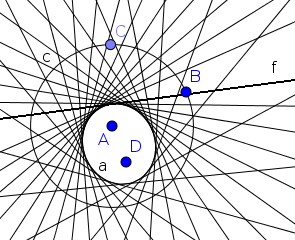
\includegraphics[scale=0.5]{Envelope-example}
\end{center}
\begin{enumerate}
    \item Mit dem \textit{Kreis mit Mittelpunkt durch Punkt} Werkzeug, wird ein Kreis $c$ mit dem Mittelpunkt $A$und dem Umkreispunkt $B$ konstruiert.
    \item Setzen Sie Punkt $C$ auf $c$.
    \item Erstellen Sie einen beliebigen Punkt $D$ in $c$.
    \item Konstruieren Sie die \textit{Mittelsenkrechte} $f$ der Strecke $CD$ unter Verwendung der Endpunkte.
    \item Geben Sie \texttt{Einhüllende[f,C]}in der Befehlszeile ein. Die implizite Kurve $a$ wird berechnet und gezeichnet. Diese sieht aus wie eine Ellipse.
\end{enumerate}


\subsection{Technische Notizen}

Die folgenden Notizen sind wichtige Einschränkungen für jedes Automatische Begründungswerkzeug in GeoGebra, symbolische Berechnungen nutzt:
\begin{itemize}
\item Es werden nicht alle GeoGebra Werkzeuge und Konstruktionsschritte unterstützt.
\item Die unterstützten Werkzeuge funktionieren nur für eine beschränkte Menge an geometrischen Objekten, zum Beispiel die Verwendung von Punkten, Geraden, Kreisen, Kegel.
\item Abschnitte von Strahlen und Geraden werden als unendliche Geraden behandelt. Kreisbögen werden wie Kreise behandelt.
\item Zu komplizierte Ortslinien- oder Einhüllende-Berechnungen können in der Algebra Ansicht als "undefiniert" dargestellt werden.
\item Beziehungs-Beweise, deren Inhalt zu kompliziert ist, werden die Mitteilung "möglicherweise allgemein wahr" anzeigen. Die Interpretation dafür ist, dass es GeoGebra nicht möglich ist, zu entscheiden, ob die Beziehung im allgemeinen wahr ist, aber die numerischen Ergebnisse lassen darauf schließen.
Das heißt, die Beziehung kann auch im allgemeinen falsch sein.
\item Wenn es keine Ortslinie oder Einhüllende gibt, ist die implizite Kurve die leere Menge $0=1$. Zum Beispiel: Für einen beliebigen Punkt $P$
\begin{center}
\texttt{Ortsliniengleichung[false,P]}
\end{center}
zeigt die leere Menge.
\item Wennn die Ortslinie oder die Einhüllende die ganze Ebene ist, hat die implizite Kurve die Gleichung $0=0$. Zum Beispiel: Für einen beliebigen Punkt $P$
\begin{center}
\texttt{Ortsliniengleichung[true,P]}
\end{center}
zeigt die ganze Ebene.
\item Manchmal werden zusätzliche Verzweigungen erscheinen, die nicht in der ursprünglichen Ortslinie oder Einhüllenden waren.
\item Der Graph der impliziten Kurve kann in manchen Fällen ungenau sein.
\end{itemize}

\section{Verwendung in der Klasse: Vermutung, Beweis und Verallgemeinerung}

Technisch gesehen ist das Beziehungswerkzeug das einfachsten symbolische Werkzeug aus der obigen Liste. Auf der anderen Seite können manche Unterrichtssituationen den Einsatz andere Werkzeuge, oder den Einsatz mehr als eines Werkzeuges erfordern, möglicherweise auch in einer anderen Reihung als in der obigen Liste.

\subsection{Satz des Thales}

In vielen traditionellen Mathematikstunden wird der Satz des Thales in einer expliziten Form unterrichtet: Wenn $C$ auf einem Halbkreis liegt, sind die Strecken $g$ und $h$ normal aufeinander. Tatsächlich kann dieser Lehrsatz mit einer offenen Frage formuliert werden: \textit{Sei $ABC$ ein beliebiges Dreieck. Was ist die geometrische Ortslinie von $C$, wenn der Winkel bei $C$ ein rechter Winkel sein soll?}

Bei diesem Zugang kann es sinnvoller sein, den technisch anspruchsvolleren \texttt{Ortsliniengleichung[g$\perp$h,C]} Befehl zuerst zu verwenden und dann die Konstruktion mit dem Beziehungswerkzeug oder -befehl zu vollenden. Der Output des   \texttt{Ortsliniengleichung} Befehl kann den Schülerinnen und Schülern zeigen, dass die Kurve ein Kreis ist. Die Algebra Ansicht zeigt die Gleichung der Kurve, das könnte unter Umständen für jüngere Schülerinnen und Schüler verwirrend sein.

Schließlich kann der Satz des Thales durch das eingeschriebene Dreieck in einen Halbkreis verallgemeinert werden. In diesem Fall ist die Bedingung nicht mehr $g\perp h$, sondern der Winkel der beiden veränderlichen Strecken zu einer fixen. GeoGebra unterstützt diese Art der Erhebung mit der Schreibweise.
\begin{center}
\texttt{Ortsliniengleichung[SindKongruent[$\alpha$,$\beta$],C]}
\end{center}
wenn $\alpha$ fix ist und $\beta=\angle{ACB}$.

Zusammenfassend, bei diesem Zugang
\begin{enumerate}
    \item wird eine implizite Ortslinie mit GeoGebra berechnet,
    \item wird von den Schülerinnen und Schülern eine Vermutung aufgestellt, wie die Kurve aussieht,
    \item wird die Vermutung mit dem Beziehungswerkzeug oder -befehl in GeoGebra überprüft,
    \item kann der Beweis von den Schülerinnen und Schülern optional handschriftlich durchgeführt werden,
    \item wird der Satz des Thales mit den impliziten Ortslinien in GeoGebra verallgemeinert - als zukünftiges Experiment für die Schülerinnen und Schüler.
\end{enumerate}

\subsection{weitere Beispiele}

Die Dreiecksungleichung kann in eine Gleichung übersetzt werden, die in eine Erforschung der degenerierten Dreiecke geändert werden kann. Als Verallgemeinerung kann die künstliche Definition von konischen Segmenten erwähnt werden.

Eine andere Anwendung ist eine Verzweigung der Ortsliniengleichung im Dreieck $ABC$ mit der Bedingung $a\stackrel{?}{=}b$, dazu muss $C$ gefunden werden (step 1). Natürlich muss $C$ auf der Streckensymmetrale  $AB$ liegen (step 2). Dass  $C$ explizit auf der Streckensymmetrale liegt, bestätigt GeoGebra, als $AC=BC$ , wenn man die Berechnung mit dem Beziehungswerkzeug startet (step 3). Nach dem Beweis des Satzes mit traditionellen Methoden (step 4) kann eine Verallgemeinerung durch das Eintippen des Befehles\texttt{Ortsliniengleichung[a==2b,C]}: erhalten werden. Dies kann auch ein interessantes Experiment für fortgeschrittene Schülerinnen und Schüler sein. (step 5).

\subsection{Ein ausgearbeitetes Beispiel: Das A worked out example: The midline theorem}

Here step-by-step instructions are provided on a possible way on investigating the midline theorem by using GeoGebra's automated reasoning tools.

\paragraph{Step 1}
\begin{center}
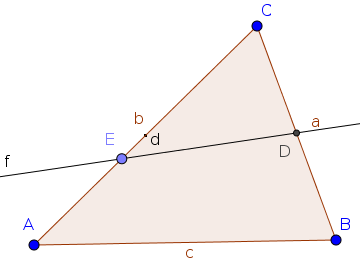
\includegraphics[scale=0.5]{classroom1}
\end{center}
\begin{enumerate}
    \item By using the \textit{Polygon} tool, construct triangle $ABC$. This will automatically create segments $a$, $b$ and $c$.
    \item By using the \textit{Midpoint or Center} tool, create the midpoint $D$ of $a$.
    \item Put point $E$ on $b$.
    \item Create line $f$ which joins $D$ and $E$.
    \item Ask GeoGebra on the requirement for $E$ in order to have $f$ parallel to $c$: type \texttt{LocusEquation[c$\parallel$f,E]} in the Input Bar. Now the implicit curve $d$ will be computed and plotted, and it seems to be a single point. Note: it may to be useful to change the line thickness of the implicit curve $d$, and also to increase ist layer number to ensure that other objects do not hide it. Both settings can be changed in the Object properties window.
\end{enumerate}
\paragraph{Step 2}
\begin{center}
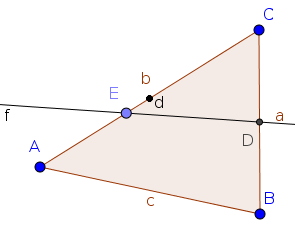
\includegraphics[scale=0.5]{classroom2}
\end{center}
\begin{enumerate}
    \item[6.] Drag the free objects and conjecture that $E$ must be the midpoint of $b$.
    \item[7.] To confirm this conjecture create midpoint $F$ of segment $b$ (and align labels of $d$ and $F$ to avoid overlapping). Drag the free objects again.
\end{enumerate}
\paragraph{Step 3}
\begin{center}
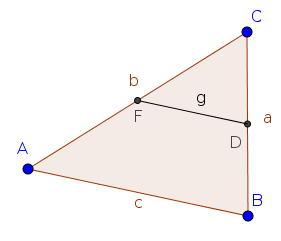
\includegraphics[scale=0.5]{classroom3}
\end{center}
\begin{enumerate}
    \item[8.] Make the objects $E$, $f$ and $d$ invisible by hiding them.
    \item[9.] Join $D$ and $F$ by segment $g$.
    \item[10.] Use the \textit{Relation} tool to compare $c$ and $g$. They seem to be parallel.
    \item[11.] Click ``More$\ldots$'' in the popup window and check symbolically that they are indeed parallel.
\end{enumerate}
\begin{center}
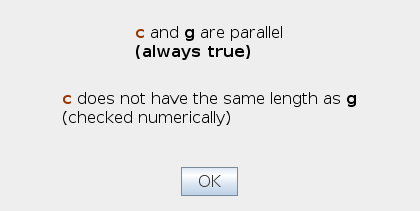
\includegraphics[scale=0.5]{classroom3-Relation}
\end{center}
The pupils may continue with step 4 if they need an elegant way to prove this statement, or just stop here if there is no time for further work in the classroom.

Also, in step 5 further questions can be raised. $c$ and $g$ do not have the same length---but can $g$ be computed by using the length of $c$? Maybe $c=1.5\cdot g$, or maybe more? The GeoGebra command \texttt{Relation[c,1.5g]} will result in the answer that $c$ and $1.5g$ are not equal, but maybe there is another constant than $1.5$ which results in a positive answer$\ldots$ Even if there is no time for further work in the classroom, some pupils may find these questions interesting and they can continue thinking on them alone or in groups---but in some sense \textit{independently}, using the computer as an expert system.

\section{Limitations: a case study of Thales' circle theorem}

Intiutive use of GeoGebra Automated Reasoning Tools may result in unexpected outputs in some cases. This subsection explains some common mistakes during their use.

Different approaches will be discussed when investigating Thales' circle theorem.

\paragraph{Approach 1}
\begin{center}
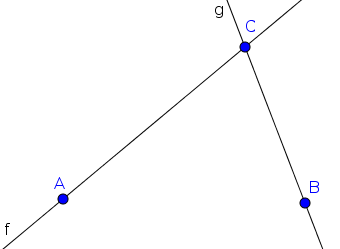
\includegraphics[scale=0.5]{limitations-Thales1-1}
\end{center}
\begin{enumerate}
    \item Create points $A$, $B$ and $C$.
    \item Create lines $f=AC$, $g=BC$.
    \item Check the result of the command \texttt{Relation[f,g]}: ``$f$ intersects with $g$''.
    \item Ask GeoGebra about geometric prerequisites of $f\perp g$:
\begin{center}\texttt{LocusEquation[f$\perp$g,C]}.\end{center}
An implicit curve $a$ which seems like a circle will be shown.
    \item Move $C$ in the neighborhood of the implicit curve as close as possible. Now \texttt{Relation[f,g]} may still report that ``$f$ intersects with $g$''. \textbf{Why? Because the point $C$ may be not accurately on the circle. We need to exactly state that it is on the circle.}
    \begin{enumerate}
      \item Try attaching point $C$ on implicit curve $a$ by using the \textit{Attach / Detach Point} tool. \textbf{This is not allowed in GeoGebra, because by definition $a$ depends on $C$, and circular dependency would make no sense.}
      \item Instead, create a new point $D$ by putting it on the implicit curve. This is allowed in GeoGebra. Create also lines $h=AD$, $i=BD$.
\begin{center}
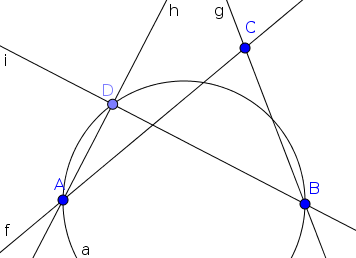
\includegraphics[scale=0.5]{limitations-Thales1-2}
\end{center}
      \item Check the result of the command \texttt{Relation[h,i]}: ``$h$ and $i$ are perpendicular'' when checked numerically. By clicking ``More$\ldots$'' the result is however ``possibly generally true''. \textbf{Why? Because GeoGebra interprets the underlying implicit curve as the result of a particular setup of the construction. In other words: an implicit curve is a numerical object, it does not have a symbolic representation. That is, symbolic checks based on an implicit curve are not possible. Here GeoGebra was just optimistic about the truth of the conjecture, but the software was actually unable to prove it.}
      \item The proper way to finalize the steps in this approach is to create the circle with diameter $AB$ with a Circle tool, for example by using the \textit{Semicircle through 2 Points} tool, after detaching $D$ from $a$ and making $a$ invisible. Now $D$ can be attached to the semicircle.
\begin{center}
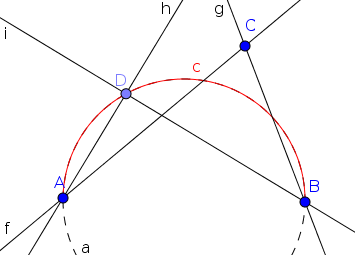
\includegraphics[scale=0.5]{limitations-Thales1-3}
\end{center}
      (Optionally the implicit curve can be set to visible by displaying it with a different style. In this example another style was used for the semicircle as well.) Finally \texttt{Relation[h,i]} will now result in positive outputs both numerically and symbolically.
    \end{enumerate}
\end{enumerate}


\paragraph{Approach 2}
\begin{center}
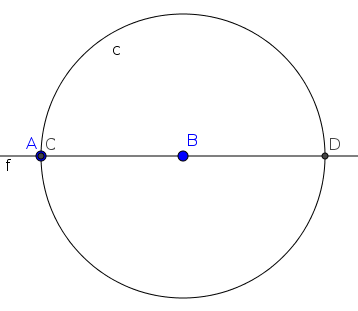
\includegraphics[scale=0.5]{limitations-Thales2-1}
\end{center}
\begin{enumerate}
    \item Create points $A$ and $B$.
    \item Create circle $c$ with center $B$ through $A$.
    \item Draw line $f$ by joining points $A$ and $B$.
    \item Create the intersection points $C$ and $D$ of $c$ and $f$. (You may want to move the label of $A$ away to avoid overlapping with the label of $C$.)
    \item Put point $E$ on $c$.
    \item Draw lines $g=AE$, $h=DE$.
\begin{center}
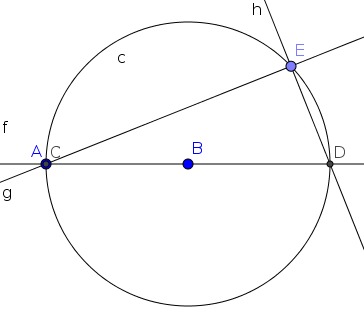
\includegraphics[scale=0.5]{limitations-Thales2-2}
\end{center}
    \item Compare $g$ and $h$ by using \texttt{Relation[g,h]}. The numerical result is correct, but GeoGebra reports that the perpendicularity of $f$ and $g$ is not generally true. \textbf{Why? When $C$ and $D$ were created, it was not defined which is which. That is, the visual precondition that $A=C$ is actually false---the other case $A=D$ must be also allowed as a possible precondition. In that other case, of course, $f$ and $g$ are not perpendicular, but identical.}
\begin{enumerate}
      \item Instead, change the definition of $g$ to $g=CE$. Now the relationship between $g$ and $h$ will be correctly reported in the symbolic case as well.
      \item Another option is to not create both intersection points $C$ and $D$, but just one of them (which differs from $A$). This is possible by clicking on the neighborhood of the sought intersection point in the diagram.
\begin{center}
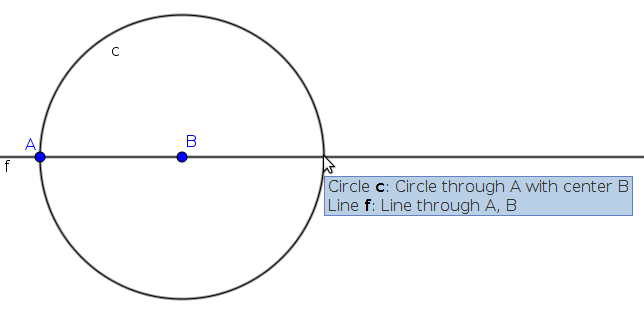
\includegraphics[scale=0.5]{limitations-Thales2-3}
\end{center}
      Now continuing with the creation of $D$ (by putting it on $c$), $g=AD$ and $h=CD$, \texttt{Relation[f,g]} will report the correct results both numerically and symbolically.
\begin{center}
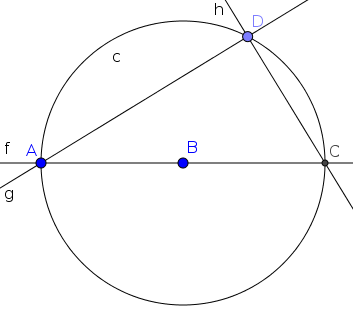
\includegraphics[scale=0.5]{limitations-Thales2-4}
\end{center}
      \textbf{Why? In this diagram GeoGebra assumes that $C$ differs from $A$ in general (the special case $A=C$ will be excluded from the symbolic proof of the perpendicularity---but even in this side case the statement on perpendicularity will be true, that is the symbolic result will be ``always true'').}
    \end{enumerate}
\end{enumerate}


\section{Appendix}
\subsection{Low level GeoGebra tools}

Automated reasoning tools in GeoGebra are completed by some low level tools prepared for learning more and in a more accurate way about geometric properties.

\subsubsection{The \texttt{Prove} command}
The \texttt{Prove} command decides if a geometric statement is true in general. It has three possible outputs:
\begin{itemize}
    \item \textit{true} means that the statement is always true, or true under some non-degeneracy conditions.
    \item \textit{false} means that the statement is false in general. GeoGebra uses algebraic geometry in many cases to decide such questions. In algebraic geometry ``generally true'' (true in ``most'' cases) and ``generally false'' (false in ``most'' cases) are not opposite properties, that is, a statement can be not ``generally true'' and not ``generally false'' at the same time. GeoGebra interprets this special case as \textit{false} (since it is not generally true).
    \item \textit{undefined} means that GeoGebra cannot decide because of some reason:
    \begin{itemize}
        \item The statement cannot be translated into a model which can be further investigated. This usually means that algebraization of the statement failed because of 
        \begin{itemize}
            \item theoretical impossibility (e.g.~using a transcendent function as a construction step, for example, sine of $x$),
            \item missing implementation in GeoGebra.
        \end{itemize}
        \item The translated statement in algebraic geometry is too difficult to solve. This means that either there are too many variables, or the equations are hard to handle by the solver algorithm. This results in either a timeout or an out of memory error.
        \item The solver algorithm was able to investigate the situation, but the result is ambiguous: either the statement is false, or it is true under certain conditions---but the algorithm was not able decide which case is present.
        \item There was an internal error in GeoGebra during the computations.
    \end{itemize}
\end{itemize}

% Prevent putting the image on the next page.
\vfill\eject % FIXME

\paragraph{Example}
\begin{center}
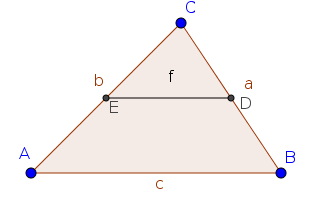
\includegraphics[scale=0.5]{Prove-example}
\end{center}
\begin{enumerate}
\item Construct the triangle $ABC$ by using the \textit{Polygon} tool.
\item Construct the midpoints $D$ and $E$ of sides $a$ and $b$, respectively, by using the \textit{Midpoint or Center} tool.
\item By using the \textit{Segment} tool, create $f$ by joining $D$ and $E$.
\item Type \texttt{Prove[f$\parallel$c]} to obtain \textit{true} in the Algebra View as Boolean Value $d$. Note that the parallel sign must be entered by using either
\begin{itemize}
\item the list of the mathematical symbols by clicking the \framebox{$\alpha$} icon in the Input Bar, or
\item inserting this symbol externally by using Copy and Paste.
\item Alternatively, \texttt{f$\parallel$c} can be substituted by \texttt{AreParallel[f,c]} also.
\end{itemize}

\item Type \texttt{Prove[c==3f]}. Now the answer is \textit{undefined}, because GeoGebra cannot decide if the statement is false or it is true under certain conditions. In such cases the \texttt{ProveDetails} command can help (see below). Note that \textit{two} equal signs must be entered; another possibilities are to use
\begin{itemize}
    \item \texttt{Prove[c$\stackrel{?}{=}$3f]}, or
    \item \texttt{Prove[AreEqual[c,3f]]}.
\end{itemize}

\end{enumerate}

\subsubsection{The \texttt{ProveDetails} command}
The \texttt{ProveDetails} command has similar behavior like the \texttt{Prove} command has, but it may use different algorithms in the decision process, and may provide more information on the results. It has three possible outputs:
\begin{itemize}
    \item \textit{\{true\}} means that the statement is always true.
    \item \textit{\{true, \{$\ldots$\}\}} if the statement is true under some non-degeneracy or essential conditions: these conditions are listed in the internal braces. (If the list remains ``$\ldots$'', it means that no synthetic translation could be found.)  If the conjunction of the negated conditions is true, then the statement is true.
    \item \textit{\{false\}} means that the statement is false in general. See the comments at the \texttt{Prove} command for more details on this.
\end{itemize}
\paragraph{Example (continued)}
\begin{enumerate}
\setcounter{enumi}{5}
    \item Type \texttt{ProveDetails[c==3f]}. Now the answer is \textit{\{false\}}.
    \item Type \texttt{ProveDetails[c==2f]}. Now the answer is \textit{\{true\}}.
\begin{center}
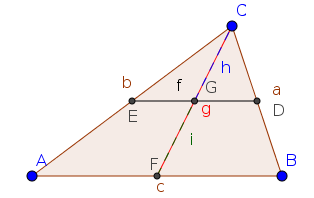
\includegraphics[scale=0.5]{ProveDetails-example-1}
\end{center}
    \item Now let $F$ be the midpoint of $c$, and let us denote segment $CF$ by $g$. Let $G$ be the intersection point of $f$ and $g$. Finally, let us denote segments $CG$ and $FG$ by $h$ and $i$, respectively. In this case \texttt{ProveDetails[h==i]} returns \textit{\{true,\{``AreCollinear[A,B,C]''\}\}} which means that if $A$, $B$ and $C$ are not collinear, then $h=i$.
\end{enumerate}

\paragraph{Another example}
\begin{center}
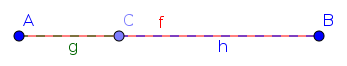
\includegraphics[scale=0.5]{ProveDetails-example-2}
\end{center}
\begin{enumerate}
    \item Let $AB$ a segment, denoted by $f$.
    \item Let $C$ be a point on $f$.
    \item Let us denote segments $AC$ and $BC$ by $g$ and $h$, respectively.
    \item Type \texttt{ProveDetails[f==g+h]}. Now the answer is
    \begin{center}
        \textit{\{true,\{``g+f=h'', ``h+f=g''\}\}} 
    \end{center}
    which means that if $g+f\neq h$ and $h+f\neq g$, then $f=g+h$.
\end{enumerate}

\subsubsection{A comparison of \texttt{Prove}, \texttt{ProveDetails} and \texttt{Relation}}
\label{Erklaerungstabelle}

The following table explains the meanings of the outputs of the commands \texttt{Prove},
\texttt{ProveDetails} and \texttt{Relation}.

% This table was exported from LyX. LaTeX experts: Please improve its look if possible.
\begin{tabular}{|>{\raggedright}m{0.15\textwidth}|>{\centering}m{0.2\textwidth}|>{\centering}m{0.2\textwidth}|>{\centering}m{0.3\textwidth}|}
\hline 
\multicolumn{3}{|c|}{GeoGebra outputs} & \multirow{2}{0.3\textwidth}{\textbf{\centerline{Conclusion}}}\tabularnewline
\cline{1-3} 
\textbf{\centerline{Prove}} & \textbf{ProveDetails} & \textbf{Relation}'s symbolic window & \tabularnewline
\hline 
\multirow{4}{0.15\textwidth}{\centerline{\footnotesize{}true}} & {\footnotesize{}\{true\}} & {\footnotesize{}always true} & {\footnotesize{}The statement is true.}\tabularnewline
\cline{2-4} 
 & \multicolumn{1}{>{\centering}m{0.2\columnwidth}|}{{\footnotesize{}\{true,\{}\emph{\footnotesize{}conditions}{\footnotesize{}\}\}}} & {\footnotesize{}true under }\emph{\footnotesize{}conjuction of specified
conditions} & {\footnotesize{}The statement is true if the specified }\emph{\footnotesize{}conditions}{\footnotesize{}
hold. These conditions are sufficient, but maybe not necessary. There
may be other sufficient conditions to make the statement true.}\tabularnewline
\cline{2-4} 
 & {\footnotesize{}\{true,\{$\ldots$\}\}} & {\footnotesize{}true under certain conditions} & {\footnotesize{}The statement is true if certain equations hold. These
equations have no visually clear geometric meanings for GeoGebra.}\tabularnewline
\cline{2-4} 
 & {\footnotesize{}\{\}} & {\footnotesize{}generally true} & {\footnotesize{}The statement is true if certain conditions hold.
GeoGebra was unable to find these conditions due to computational
difficulties.}\tabularnewline
\hline 
\multirow{2}{0.15\textwidth}{\centerline{\footnotesize{}false}} & {\footnotesize{}\{false\}} & {\footnotesize{}not generally true} & {\footnotesize{}The statement is false.}\tabularnewline
\cline{2-4} 
 & {\footnotesize{}\{\}} & {\footnotesize{}possibly generally true} & {\footnotesize{}GeoGebra was unable to decide if the statement is
true or false. The numerical check confirms the truth, but the symbolic
check was unsuccessful due to computational difficulties.}\tabularnewline
\hline 
\multirow{5}{0.15\textwidth}{\centerline{\footnotesize{}undefined}} & {\footnotesize{}\{true\}} & {\footnotesize{}always true} & {\footnotesize{}The statement is true.}\tabularnewline
\cline{2-4} 
 & \multicolumn{1}{c|}{{\footnotesize{}\{true,\{}\emph{\footnotesize{}conditions}{\footnotesize{}\}\}}} & {\footnotesize{}true under }\emph{\footnotesize{}conjuction of specified
conditions} & {\footnotesize{}The statement is true if the specified }\emph{\footnotesize{}conditions}{\footnotesize{}
hold. These conditions are sufficient, but maybe not necessary. There
may be other sufficient conditions to make the statement true.}\tabularnewline
\cline{2-4} 
 & {\footnotesize{}\{true,\{$\ldots$\}\}} & {\footnotesize{}true under certain conditions} & {\footnotesize{}The statement is true if certain conditions hold.
These equations have no visually clear geometric meanings for GeoGebra.}\tabularnewline
\cline{2-4} 
 & {\footnotesize{}\{false\}} & {\footnotesize{}generally false} & {\footnotesize{}The statement is false.}\tabularnewline
\cline{2-4} 
 & {\footnotesize{}\{\}} & {\footnotesize{}possibly generally true} & {\footnotesize{}GeoGebra was unable to decide if the statement is
true or false. The numerical check confirms the truth, but the symbolic
check was unsuccessful due to computational difficulties, or the symbolic
check for the given statement is not yet implemented in GeoGebra.}\tabularnewline
\hline 
\end{tabular}


\subsection{Debugging}
Starting GeoGebra via command line there are more possibilities to investigate the results. Here the method on a typical Linux installation is demonstrated.

The user needs to start GeoGebra by the following command:
{
%\scriptsize
    \begin{center}
        \texttt{geogebra --logfile=/dev/stdout --logshowcaller=false $\backslash$\\ --logshowtime=false --logshowlevel=false} 
    \end{center}
} % \scriptsize
A typical output looks like as follows:
{
\scriptsize
\begin{lstlisting}[language=mylog]
Using AUTO
Using BOTANAS_PROVER
A = (3.42, 1.86) /* free point */
// Free point A(v1,v2)
B = (10.48, 3.1) /* free point */
// Free point B(v3,v4)
f = Segment[A, B] /* Segment [A, B] */
C = Point[f] /* Point on f */
// Constrained point C(v5,v6)
Hypotheses:
1. -v5*v4+v6*v3+v5*v2-v3*v2-v6*v1+v4*v1
g = Segment[A, C] /* Segment [A, C] */
h = Segment[C, B] /* Segment [C, B] */
Processing numerical object
Hypotheses have been processed.
giac evalRaw input: evalfa(expand(ggbtmpvarf))
giac evalRaw output: ggbtmpvarf
input = expand(ggbtmpvarf)
result = ggbtmpvarf
eliminate([ggbtmpvarf-((ggbtmpvarg)+(ggbtmpvarh))=0,ggbtmpvarh^2=v11^2,ggbtmpvarg^2=v12^2,ggbtmpvarf^2=v13^2],[ggbtmpvarh,ggbtmpvarg,ggbtmpvarf])
giac evalRaw input: evalfa(eliminate([ggbtmpvarf-((ggbtmpvarg)+(ggbtmpvarh))=0,ggbtmpvarh^2=v11^2,ggbtmpvarg^2=v12^2,ggbtmpvarf^2=v13^2],[ggbtmpvarh,ggbtmpvarg,ggbtmpvarf]))
Running a probabilistic check for the reconstructed Groebner basis. If successfull, error probability is less than 1e-07 and is estimated to be less than 10^-18. Use proba_epsilon:=0 to certify (this takes more time).
// Groebner basis computation time 0.000448 Memory -1e-06M
giac evalRaw output: {v11^4-2*v11^2*v12^2+v12^4-2*v11^2*v13^2-2*v12^2*v13^2+v13^4}
input = eliminate([ggbtmpvarf-((ggbtmpvarg)+(ggbtmpvarh))=0,ggbtmpvarh^2=v11^2,ggbtmpvarg^2=v12^2,ggbtmpvarf^2=v13^2],[ggbtmpvarh,ggbtmpvarg,ggbtmpvarf])
result = {v11^4-2*v11^2*v12^2+v12^4-2*v11^2*v13^2-2*v12^2*v13^2+v13^4}
giac evalRaw input: evalfa(eliminate([ggbtmpvarf-((ggbtmpvarg)+(ggbtmpvarh))=0,ggbtmpvarh=v11,ggbtmpvarg=v12,ggbtmpvarf=v13],[ggbtmpvarh,ggbtmpvarg,ggbtmpvarf]))
Running a probabilistic check for the reconstructed Groebner basis. If successfull, error probability is less than 1e-07 and is estimated to be less than 10^-18. Use proba_epsilon:=0 to certify (this takes more time).
// Groebner basis computation time 0.000592 Memory -1e-06M
giac evalRaw output: {v11+v12-v13}
input = eliminate([ggbtmpvarf-((ggbtmpvarg)+(ggbtmpvarh))=0,ggbtmpvarh=v11,ggbtmpvarg=v12,ggbtmpvarf=v13],[ggbtmpvarh,ggbtmpvarg,ggbtmpvarf])
result = {v11+v12-v13}
giac evalRaw input: evalfa(simplify({v11^4-2*v11^2*v12^2+v12^4-2*v11^2*v13^2-2*v12^2*v13^2+v13^4}/{v11+v12-v13}))
giac evalRaw output: {v11^3-v11^2*v12+v11^2*v13-v11*v12^2-2*v11*v12*v13-v11*v13^2+v12^3+v12^2*v13-v12*v13^2-v13^3}
input = simplify({v11^4-2*v11^2*v12^2+v12^4-2*v11^2*v13^2-2*v12^2*v13^2+v13^4}/{v11+v12-v13})
result = {v11^3-v11^2*v12+v11^2*v13-v11*v12^2-2*v11*v12*v13-v11*v13^2+v12^3+v12^2*v13-v12*v13^2-v13^3}
giac evalRaw input: evalfa(factor(v11^3-v11^2*v12+v11^2*v13-v11*v12^2-2*v11*v12*v13-v11*v13^2+v12^3+v12^2*v13-v12*v13^2-v13^3))
giac evalRaw output: (v11-v12-v13)*(v11-v12+v13)*(v11+v12+v13)
input = factor(v11^3-v11^2*v12+v11^2*v13-v11*v12^2-2*v11*v12*v13-v11*v13^2+v12^3+v12^2*v13-v12*v13^2-v13^3)
result = (v11-v12-v13)*(v11-v12+v13)*(v11+v12+v13)
Trying to detect polynomial -v13-v12+v11
-v13-v12+v11 means h = f + g
Trying to detect polynomial v13-v12+v11
v13-v12+v11 means f + h = g
Trying to detect polynomial v13+v12+v11
v13+v12+v11 means f + g + h = 0, uninteresting
Thesis equations (non-denied ones):
2. v11^2-v6^2-v5^2+2*v6*v4-v4^2+2*v5*v3-v3^2
3. v12^2-v6^2-v5^2+2*v6*v2-v2^2+2*v5*v1-v1^2
4. v13^2-v4^2-v3^2+2*v4*v2-v2^2+2*v3*v1-v1^2
Thesis reductio ad absurdum (denied statement), product of factors:
(v13^4-2*v13^2*v12^2+v12^4-2*v13^2*v11^2-2*v12^2*v11^2+v11^4)*v14-1
that is,
5. -1+v14*v13^4-2*v14*v13^2*v12^2+v14*v12^4-2*v14*v13^2*v11^2-2*v14*v12^2*v11^2+v14*v11^4
substitutions: {v1=0, v2=0}
Eliminating system in 8 variables (5 dependent)
giac evalRaw input: evalfa([[ff:=\"\"],[aa:=eliminate2([v12^2-v6^2-v5^2,v11^2-v6^2-v5^2+2*v6*v4-v4^2+2*v5*v3-v3^2,-1+v14*v13^4-2*v14*v13^2*v12^2+v14*v12^4-2*v14*v13^2*v11^2-2*v14*v12^2*v11^2+v14*v11^4,v13^2-v4^2-v3^2,-v5*v4+v6*v3],revlist([v6,v11,v12,v13,v14]))],[bb:=size(aa)],[for ii from 0 to bb-1 do ff+=(\"[\"+(ii+1)+\"]: [1]:  unicode95uunicode91u1]=1\");cc:=factors(aa[ii]);dd:=size(cc);for jj from 0 to dd-1 by 2 do ff+=(\"  unicode95uunicode91u\"+(jj/2+2)+\"]=\"+cc[jj]); od; ff+=(\" [2]: \"+cc[1]);for kk from 1 to dd-1 by 2 do ff+=(\",\"+cc[kk]);od;od],[if(ff==\"\") begin ff:=[0] end],ff][5])
Running a probabilistic check for the reconstructed Groebner basis. If successfull, error probability is less than 1e-07 and is estimated to be less than 10^-7. Use proba_epsilon:=0 to certify (this takes more time).
// Groebner basis computation time 0.000249 Memory -1e-06M
giac evalRaw output: "[1]: [1]:  unicode95uunicode91u1]=1  unicode95uunicode91u2]=1 [2]: 1,1"
Considering NDG 1...
Found a better NDG score (0.0) than Infinity
Statement is GENERALLY TRUE
Benchmarking: 38 ms
STATEMENT IS TRUE (yes/no: TRUE)
OUTPUT for ProveDetails: null = {true, {"f + h = g", "h = f + g"}}
\end{lstlisting}
} % \scriptsize
There is intentionally no easier way to show the users this type of output. However, the last few lines of the debug information is available in GeoGebra in the \textit{Help} menu, by choosing \textit{About/License}, and clicking \textit{System Information}---this copies the latest debug messages into the clipboard.

\subsection{Translation of GeoGebra commands}

The names of GeoGebra automated reasoning tools may need to be translated to other languages. For example, the German translation of \texttt{Prove} can be \texttt{Pr\"ufe}.
% or \texttt{Demuestra}
To learn the translated command names the following steps are recommended:

\begin{enumerate}
\item Create a GeoGebra file which contains the required commands in the Algebra View.
\item Change the language in GeoGebra in the \textit{Options} menu by choosing \textit{Language}.
\item The command names will be automatically changed in the Algebra View.
\item Move the mouse over a command in the Algebra View and read its translated name off.
\end{enumerate}



\end{document}
